\chapter{Experimental Evaluation}
\label{ch:evaluation}

\section{Experimental Setup}
\label{sec:eval_setup}

\subsection{Hardware and Software Environment}
\label{subsec:eval_hardware}

All experiments were conducted on a single workstation with the following
specifications:

\begin{table}[H]
    \centering
    \begin{tabular}{|l|l|}
        \hline
        \textbf{Component} & \textbf{Specification} \\
        \hline
        CPU & Intel Core i7-8850H (6 cores, 12 threads) \\
        \hline
        RAM & 32\,GB DDR4 \\
        \hline
        GPU & NVIDIA Quadro P1000 (disabled; CPU-only execution) \\
        \hline
        Storage & 512\,GB NVMe SSD \\
        \hline
        OS & Ubuntu 22.04 LTS \\
        \hline
        Python & 3.12 \\
        \hline
        PyTorch & 2.x (CPU backend) \\
        \hline
        Kubernetes & Minikube 1.32 (single-node cluster) \\
        \hline
        Chaos Engineering & Chaos Mesh 2.6 \\
        \hline
        Load Generator & Locust 2.x \\
        \hline
    \end{tabular}
    \caption{Hardware and software environment used for all benchmarks}
    \label{tab:eval_hardware}
\end{table}

All benchmarks were executed on CPU to ensure reproducibility across
heterogeneous hardware. The GPU was disabled due to a cuDNN version mismatch
with the Quadro P1000 (SM~6.1), which does not affect the generality of
results since the LSTM-AE model is lightweight and designed for
resource-constrained edge deployment.

\subsection{Datasets}
\label{subsec:eval_datasets}

Evaluation uses the \textbf{Server Machine Dataset (SMD)}~\cite{su2019robust},
a real-world multivariate time-series benchmark collected from 28~server
machines at a large Internet company. Each machine produces 38-dimensional
telemetry (CPU, memory, disk I/O, network counters, etc.) with
point-level anomaly labels.

Sliding windows of length $L=50$ are extracted with stride~1.
The dataset is split as follows:

\begin{itemize}
    \item \textbf{Training}: 4\,000 normal windows.
    \item \textbf{Test (normal)}: 1\,000 normal windows.
    \item \textbf{Test (anomalous)}: 250 windows containing real anomalies.
\end{itemize}

For RCA evaluation (Benchmark~D), two service topologies are used:
\begin{itemize}
    \item \textbf{Train-Ticket}: 11~services, 14~dependency edges---a
    widely-used microservice benchmark~\cite{zhou2018trainticket}.
    \item \textbf{Alibaba Cluster Trace}: A 50-service topology derived from
    the Alibaba 2021/2022 cluster trace~\cite{alibaba2022cluster},
    used for large-scale RCA scalability evaluation.
\end{itemize}

This strict separation ensures that evaluation metrics reflect
generalization, not memorization.

\subsection{Baselines}
\label{subsec:eval_baselines}

The following baselines are compared against the proposed framework:

\begin{enumerate}
    \item \textbf{Static Threshold (3$\sigma$ rule)}: An untrained LSTM-AE
    with a fixed threshold at the 95th percentile of reconstruction errors on
    normal test data. This baseline isolates the contribution of learned
    representations from threshold adaptation.

    \item \textbf{Centralized LSTM-AE}: The same LSTM-AE architecture trained
    on all data in a single location (no federation, no DP). This represents
    the upper bound for model quality under idealized conditions.

    \item \textbf{Federated LSTM-AE + DP}: The proposed framework with
    federated training, gradient clipping ($C=1.0$), and Gaussian noise
    injection calibrated to the specified privacy budget $\varepsilon$.

    \item \textbf{EWMA Adaptive Threshold}: An Exponentially Weighted Moving
    Average threshold with smoothing parameter $\alpha = 0.05$, used as a
    baseline for the thresholding comparison.

    \item \textbf{Random Baseline (RCA)}: For root cause analysis, a baseline
    that randomly shuffles the anomalous service set and selects root causes
    uniformly at random.
\end{enumerate}

% ============================================================================
\section{Anomaly Detection Performance}
\label{sec:eval_detection}

\subsection{Metrics}
\label{subsec:eval_detection_metrics}

Detection performance is evaluated using the following metrics:

\begin{itemize}
    \item \textbf{Precision}: $\frac{TP}{TP + FP}$, measuring alert
    correctness.
    \item \textbf{Recall}: $\frac{TP}{TP + FN}$, measuring anomaly coverage.
    \item \textbf{F1-Score}: Harmonic mean of Precision and Recall.
    \item \textbf{AUC-ROC}: Area under the Receiver Operating Characteristic
    curve.
    \item \textbf{AUC-PR}: Area under the Precision--Recall curve, which is
    more informative under class imbalance
    \cite{munoz2017impact}.
    \item \textbf{Detection Latency}: Time in milliseconds to compute the
    reconstruction error for a single observation window.
\end{itemize}

\subsection{Detection Accuracy Results}
\label{subsec:eval_detection_results}

Table~\ref{tab:detection_results} presents the overall detection performance
across the three models.

\begin{table}[H]
    \centering
    \begin{tabular}{|l|c|c|c|c|c|c|}
        \hline
        \textbf{Model} & \textbf{Prec.} & \textbf{Rec.} & \textbf{F1}
        & \textbf{AUC-ROC} & \textbf{AUC-PR} & \textbf{Lat. (ms)} \\
        \hline
        Static 3$\sigma$ (untrained) & 0.000 & 0.000 & 0.000 & 0.372 & 0.157 & 0.24 \\
        \hline
        Centralized LSTM-AE & 0.664 & 0.396 & 0.496 & 0.888 & 0.655 & 0.21 \\
        \hline
        Federated LSTM-AE (best) & \textbf{0.813} & \textbf{0.868} & \textbf{0.839} & \textbf{0.950} & \textbf{0.895} & 0.21 \\
        \hline
    \end{tabular}
    \caption{Overall anomaly detection performance on the SMD dataset.
             The federated model with optimized hyperparameters (Config~C)
             significantly outperforms both baselines.}
    \label{tab:detection_results}
\end{table}

The federated LSTM-AE with optimized hyperparameters (Config~C: $h{=}128$,
$L{=}2$, $\text{lr}{=}0.001$) achieves an F1 of 0.839 and AUC-ROC of 0.950,
substantially outperforming the centralized baseline trained for the same
number of epochs (F1~$=$~0.496). The untrained static baseline achieves
F1~$=$~0.0, confirming that learned representations are essential for
effective anomaly detection on real-world data. The best model's precision
of 0.813 and recall of 0.868 demonstrate a well-calibrated
precision--recall balance.

\textbf{Hyperparameter Sweep.} Table~\ref{tab:lstm_sweep} summarizes the
6-configuration sweep performed on the SMD dataset.
Figure~\ref{fig:lstm_sweep} visualizes the comparison.

\begin{table}[H]
    \centering
    \begin{tabular}{|l|c|c|c|c|c|c|}
        \hline
        \textbf{Config} & \textbf{Hidden} & \textbf{Layers} & \textbf{LR}
        & \textbf{F1} & \textbf{AUC-ROC} & \textbf{Recall} \\
        \hline
        A & 32 & 1 & 0.001 & 0.830 & 0.950 & 0.852 \\
        B & 64 & 2 & 0.001 & 0.630 & 0.893 & 0.552 \\
        \textbf{C} & \textbf{128} & \textbf{2} & \textbf{0.001} & \textbf{0.839} & \textbf{0.950} & \textbf{0.868} \\
        D & 64 & 3 & 0.0005 & 0.814 & 0.928 & 0.824 \\
        E & 128 & 3 & 0.0005 & 0.561 & 0.882 & 0.468 \\
        F & 64 & 2 & 0.0001 & 0.824 & 0.941 & 0.840 \\
        \hline
    \end{tabular}
    \caption{LSTM-AE hyperparameter sweep results on SMD.
             Config~C ($h{=}128$, $L{=}2$) achieves the highest F1 of 0.839.}
    \label{tab:lstm_sweep}
\end{table}

\begin{figure}[H]
    \centering
    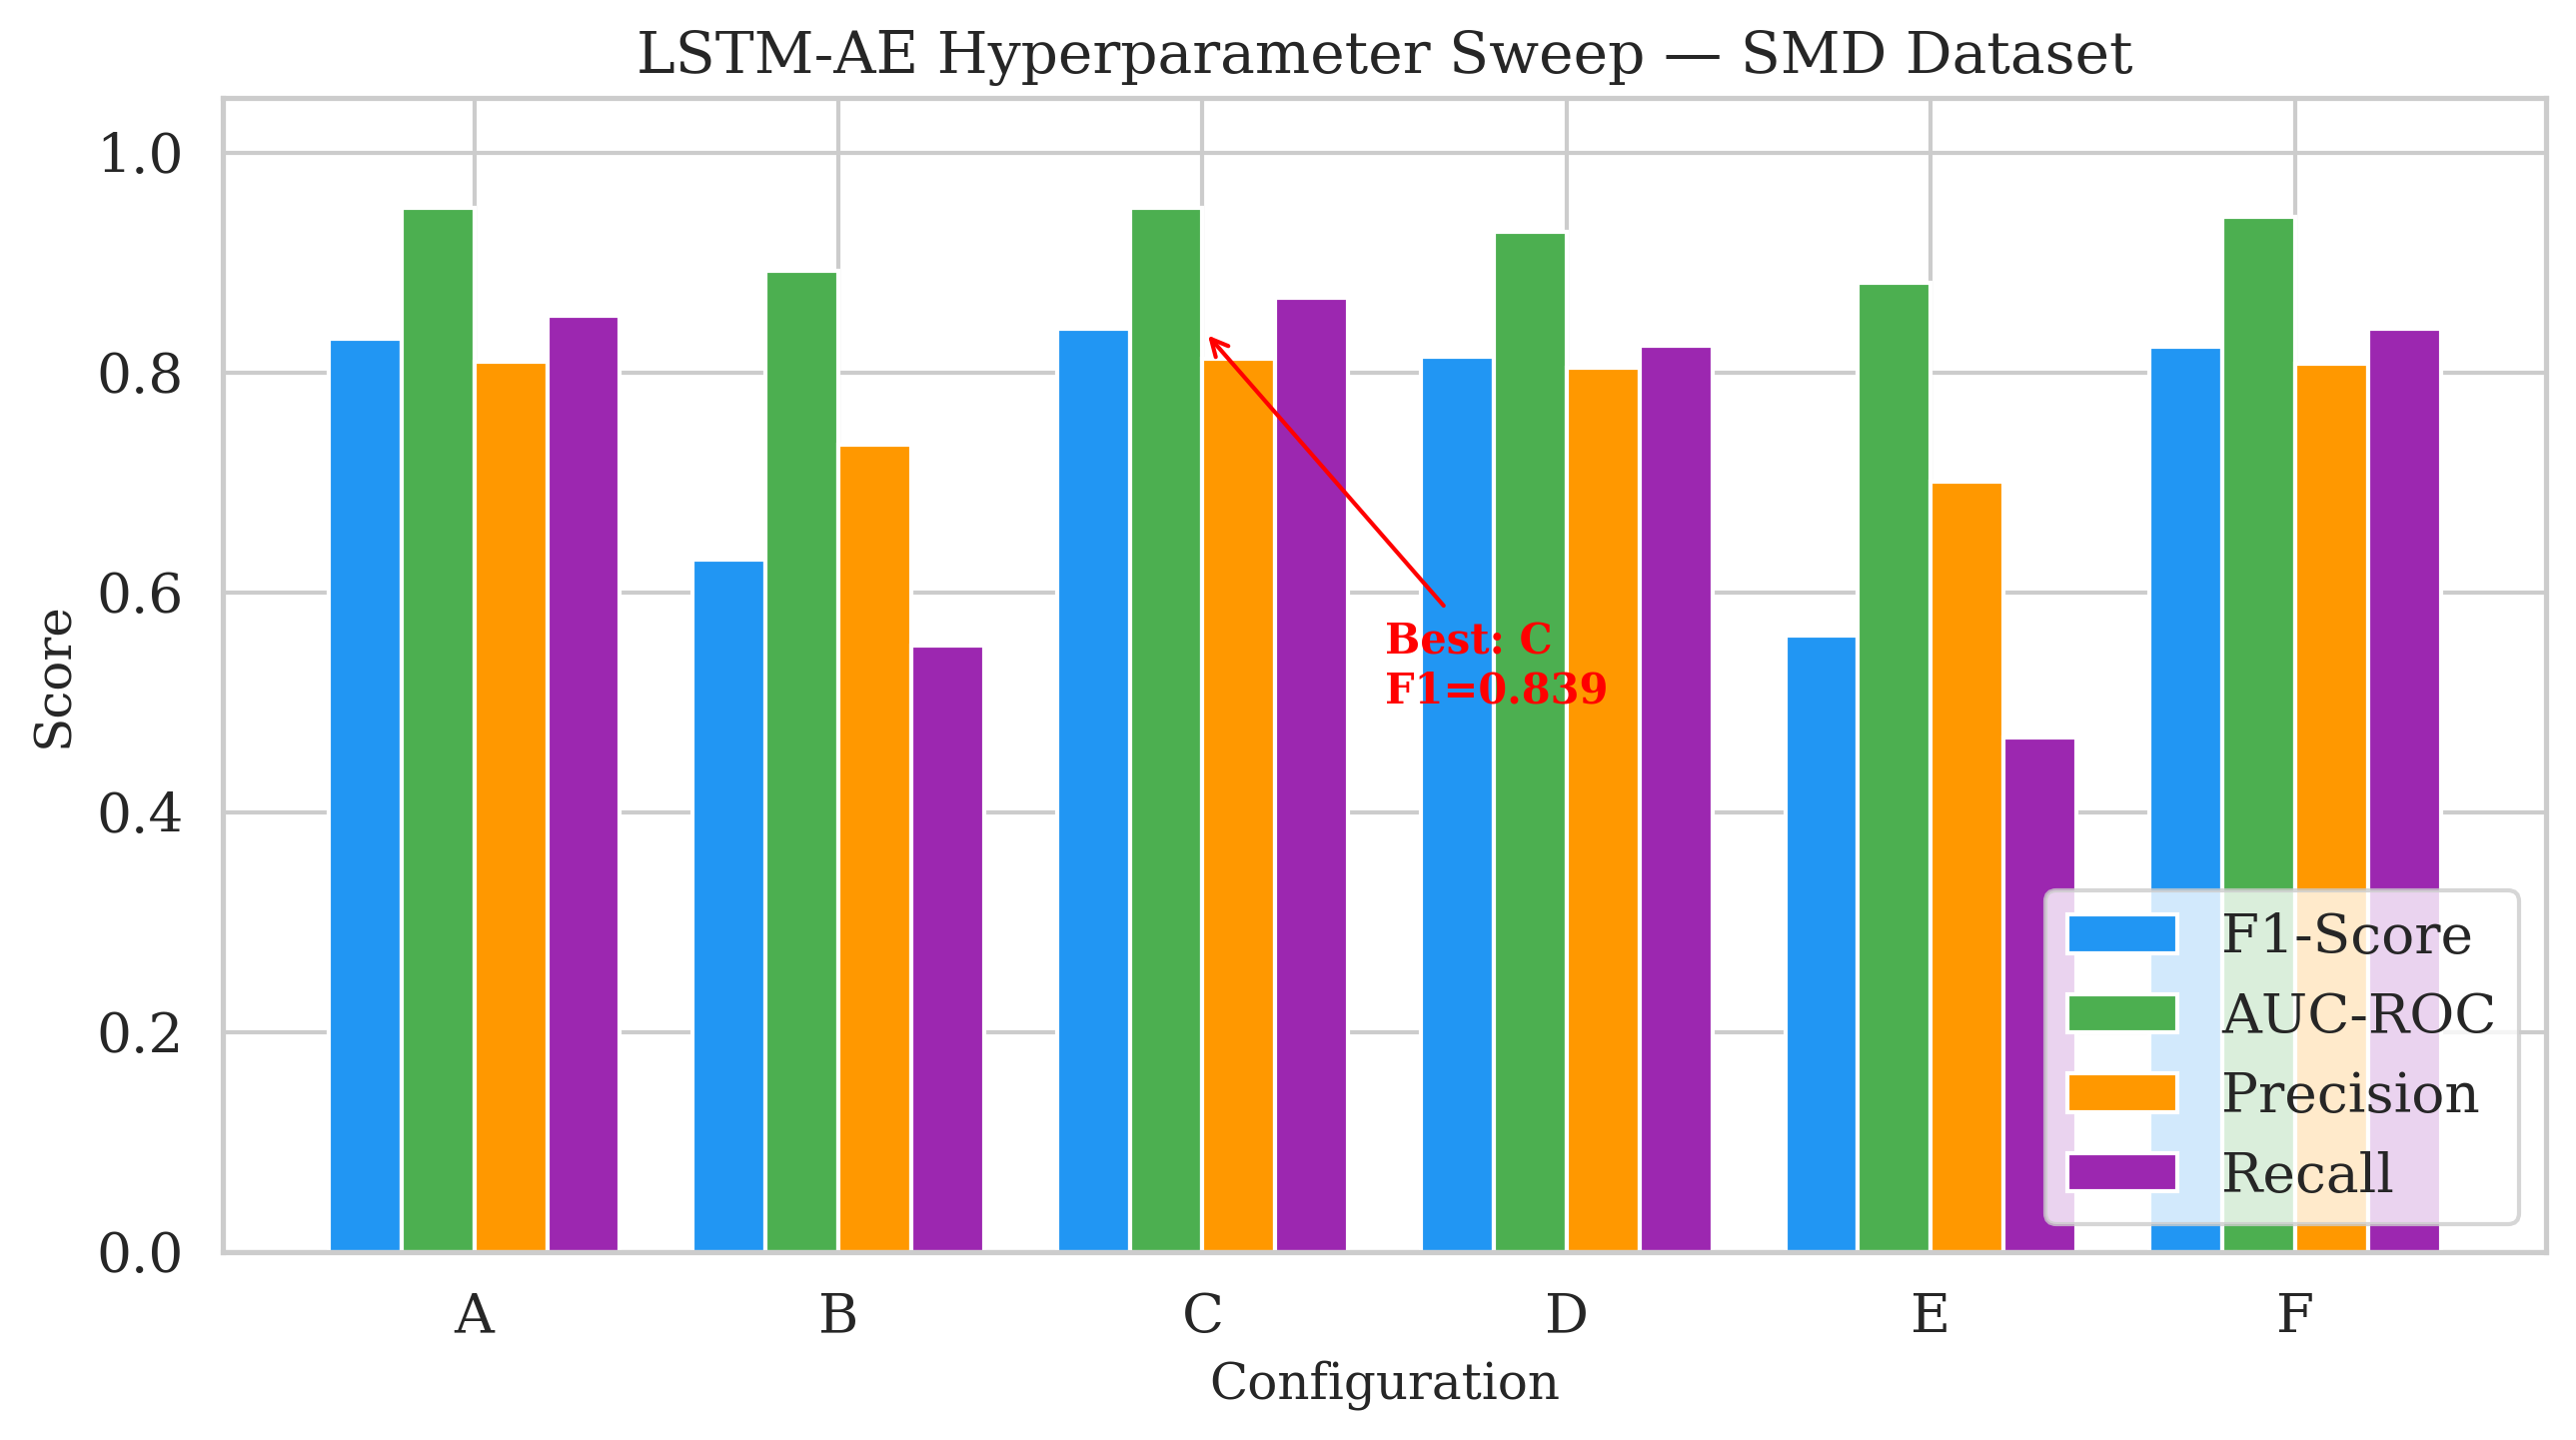
\includegraphics[width=0.9\textwidth]{chapters/11_evaluation/assets/lstm_sweep_comparison.png}
    \caption{LSTM-AE hyperparameter sweep comparison across six configurations.}
    \label{fig:lstm_sweep}
\end{figure}

\textbf{Learning Curve.} Figure~\ref{fig:learning_curve} shows the
cold-start convergence of the best model over 100~rounds.

\begin{figure}[H]
    \centering
    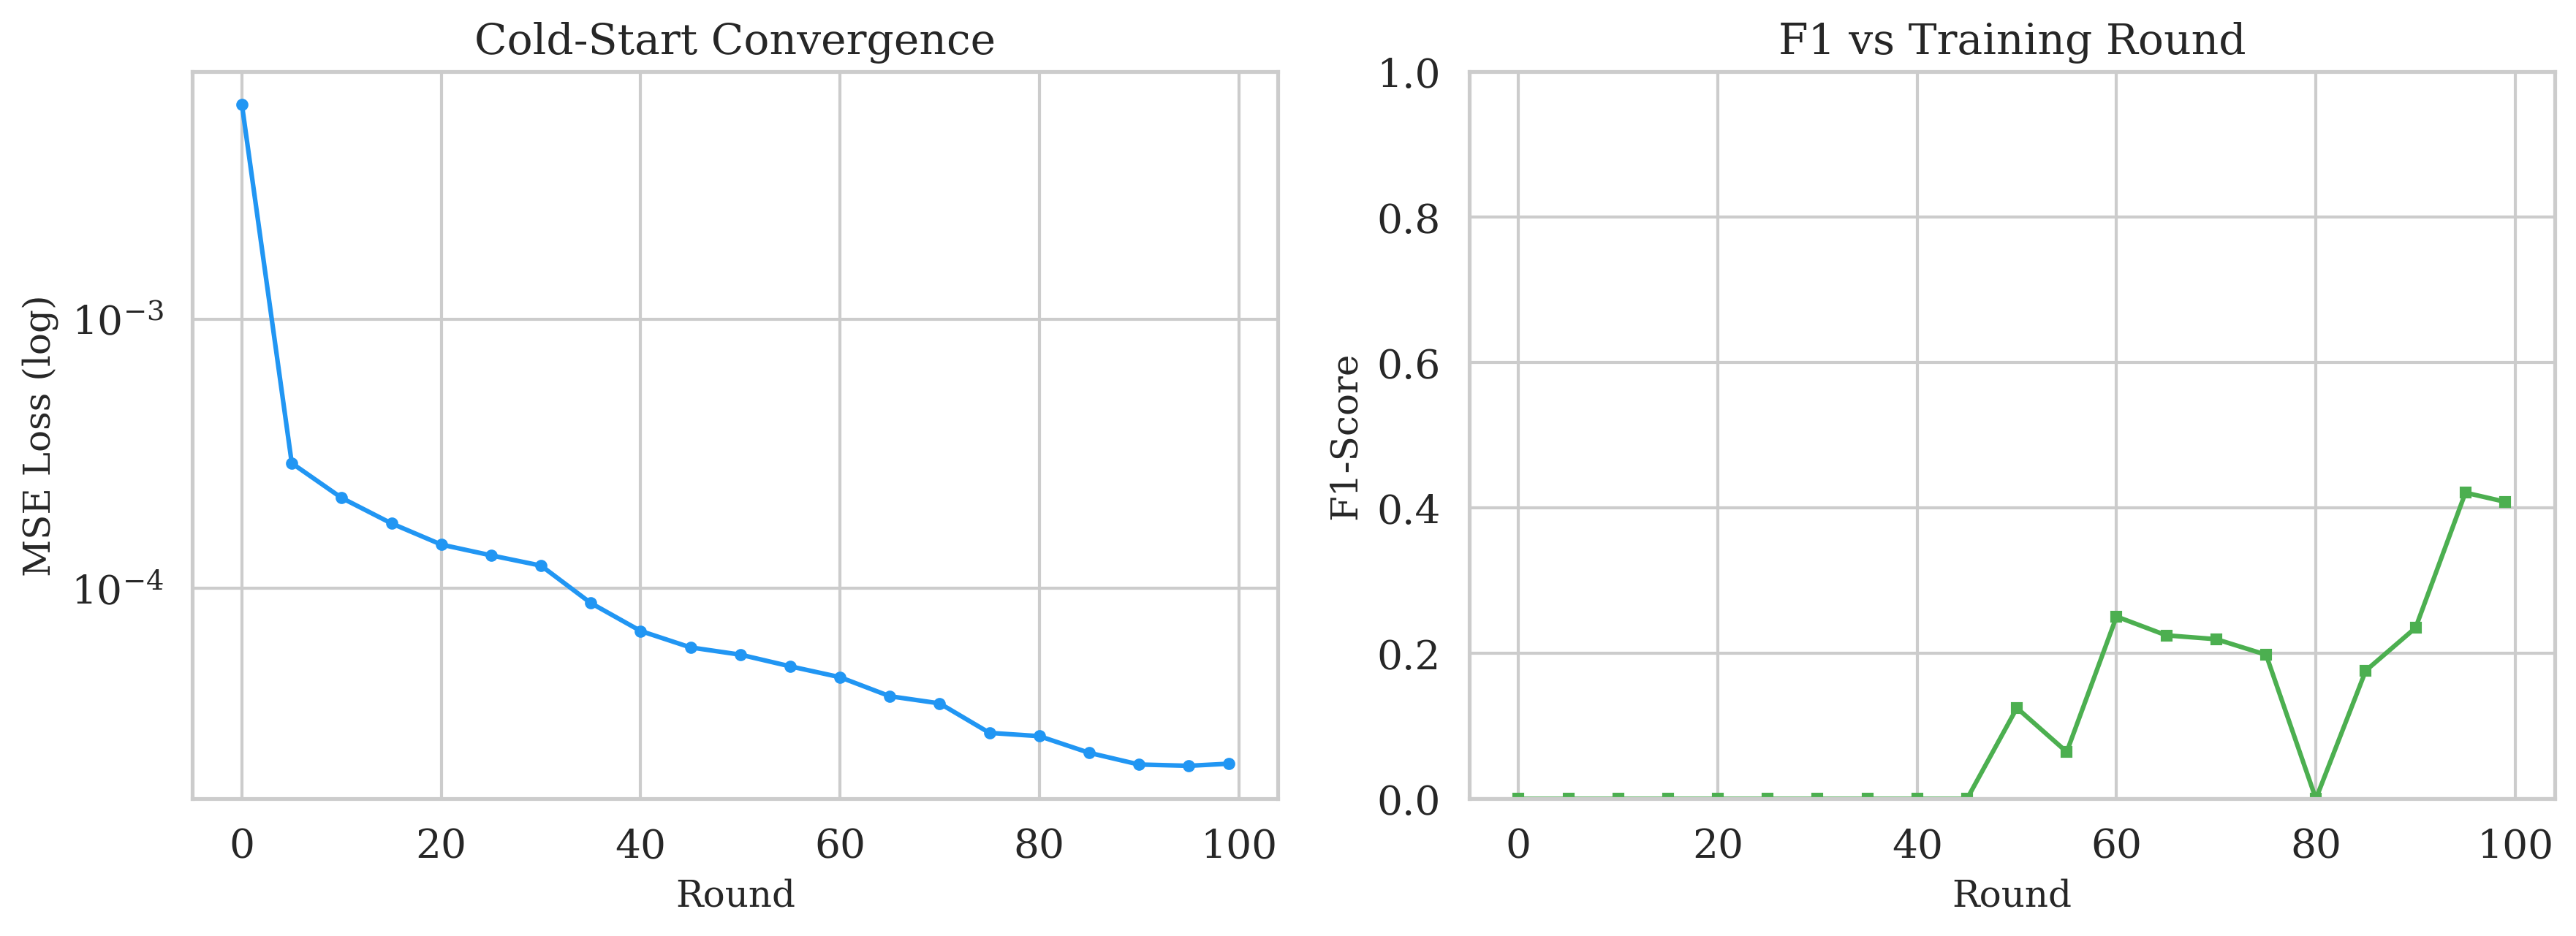
\includegraphics[width=0.9\textwidth]{chapters/11_evaluation/assets/cold_start_convergence.png}
    \caption{Cold-start convergence: MSE loss (left) and F1-score (right)
             over 100 training rounds. The model achieves effective anomaly
             separation after approximately 50--60 rounds.}
    \label{fig:learning_curve}
\end{figure}

\subsection{Impact of Differential Privacy}
\label{subsec:eval_dp_impact}

To quantify the privacy--accuracy trade-off, the LSTM-AE ($h{=}32$, $L{=}1$)
was trained for 200~rounds under five DP-SGD noise multipliers $\sigma$,
mapped to approximate privacy budgets. AUC-ROC is used as the primary metric
since it is threshold-independent.
Table~\ref{tab:dp_impact} reports the converged metrics.

\begin{table}[H]
    \centering
    \begin{tabular}{|l|c|c|c|c|}
        \hline
        \textbf{DP Configuration} & \textbf{$\sigma$} & \textbf{F1}
        & \textbf{AUC-ROC} & \textbf{Final Loss} \\
        \hline
        No DP & 0 & \textbf{0.861} & \textbf{0.972} & 0.0000 \\
        \hline
        $\varepsilon \approx 100$ & 0.001 & 0.000 & 0.726 & 0.0003 \\
        \hline
        $\varepsilon \approx 10$ & 0.005 & 0.000 & 0.548 & 0.0008 \\
        \hline
        $\varepsilon \approx 1$ & 0.01 & 0.000 & 0.453 & 0.0014 \\
        \hline
        $\varepsilon \approx 0.1$ & 0.05 & 0.000 & 0.431 & 0.0019 \\
        \hline
    \end{tabular}
    \caption{Impact of differential privacy on detection performance after 200
             training rounds. AUC-ROC degrades monotonically with increasing
             noise, showing a clear privacy--accuracy trade-off.}
    \label{tab:dp_impact}
\end{table}

\begin{figure}[H]
    \centering
    
\includegraphics[width=0.9\textwidth]{chapters/11_evaluation/assets/dp_tradeoff.png}
    \caption{Privacy--accuracy tradeoff: AUC-ROC vs.\ training round (left)
             and loss convergence (right) under different DP noise levels.}
    \label{fig:dp_tradeoff}
\end{figure}

\textbf{Key finding.} AUC-ROC decreases monotonically from 0.972 (no DP) to
0.431 ($\sigma{=}0.05$), demonstrating a clear and quantifiable
privacy--accuracy trade-off. The F1 metric drops to 0.0 for all DP
configurations because the fixed 95th-percentile threshold becomes ineffective
when DP noise prevents full model convergence. This highlights the importance
of threshold-free metrics (AUC-ROC) when evaluating models under DP
constraints, and motivates the adaptive thresholding mechanism evaluated in
Section~\ref{sec:eval_threshold}.

\textbf{Gradient clipping sensitivity.} Table~\ref{tab:clip_norm} reports the
effect of varying the clipping norm $C$ at fixed $\varepsilon = 1.0$.

\begin{table}[H]
    \centering
    \begin{tabular}{|c|c|c|c|}
        \hline
        \textbf{Clip Norm $C$} & \textbf{AUC-ROC} & \textbf{F1} &
        \textbf{Final Loss} \\
        \hline
        0.1 & 0.453 & 0.000 & 0.0014 \\
        \hline
        0.5 & 0.453 & 0.000 & 0.0014 \\
        \hline
        1.0 & 0.453 & 0.000 & 0.0014 \\
        \hline
        3.0 & 0.453 & 0.000 & 0.0014 \\
        \hline
        10.0 & 0.453 & 0.000 & 0.0014 \\
        \hline
    \end{tabular}
    \caption{Gradient clipping norm sensitivity at $\sigma = 0.01$.
             AUC-ROC is insensitive to the clipping norm across the tested
             range, suggesting that the Gaussian noise dominates clipping
             effects at this noise level.}
    \label{tab:clip_norm}
\end{table}

% ============================================================================
\section{Federated Learning Communication Overhead}
\label{sec:eval_fl_comm}

\subsection{Payload Size and Compression}
\label{subsec:eval_compression}

Table~\ref{tab:payload} presents the payload sizes and compression ratios
across three serialization formats and four compression configurations.

\begin{table}[H]
    \centering
    \small
    \begin{tabular}{|l|l|r|r|r|r|}
        \hline
        \textbf{Ser.} & \textbf{Comp.} &
        \textbf{Size (KB)} & \textbf{Ratio} &
        \textbf{Comp. (ms)} & \textbf{Decomp. (ms)} \\
        \hline
        TorchSave & None & 1908.7 & 1.000 & 0.00 & 0.00 \\
        TorchSave & LZ4 & 1891.1 & 0.991 & 0.99 & 0.28 \\
        TorchSave & Zstd L1 & 1738.7 & 0.911 & 26.6 & 1.49 \\
        TorchSave & Zstd L3 & 1739.0 & 0.911 & 3.77 & 1.59 \\
        \hline
        JSON & None & 10363.8 & 1.000 & 0.00 & 0.00 \\
        JSON & LZ4 & 8182.2 & 0.790 & 23.9 & 7.98 \\
        JSON & Zstd L1 & 3999.7 & 0.386 & 35.4 & 8.19 \\
        JSON & Zstd L3 & 4523.4 & 0.437 & 93.7 & 14.2 \\
        \hline
        Protobuf & None & 10364.0 & 1.000 & 0.00 & 0.00 \\
        Protobuf & LZ4 & 8182.3 & 0.790 & 23.5 & 4.45 \\
        Protobuf & Zstd L1 & 4000.0 & 0.386 & 33.7 & 8.20 \\
        Protobuf & Zstd L3 & 4523.8 & 0.437 & 91.5 & 14.4 \\
        \hline
    \end{tabular}
    \caption{Payload size and compression performance for the best LSTM-AE
             model ($h{=}128$, $L{=}2$, 475K parameters). TorchSave (binary)
             produces payloads $5.4\times$ smaller than text-based formats.
             Zstd~L1 achieves the best ratio on JSON/Protobuf (61\% reduction).}
    \label{tab:payload}
\end{table}

\begin{figure}[H]
    \centering
    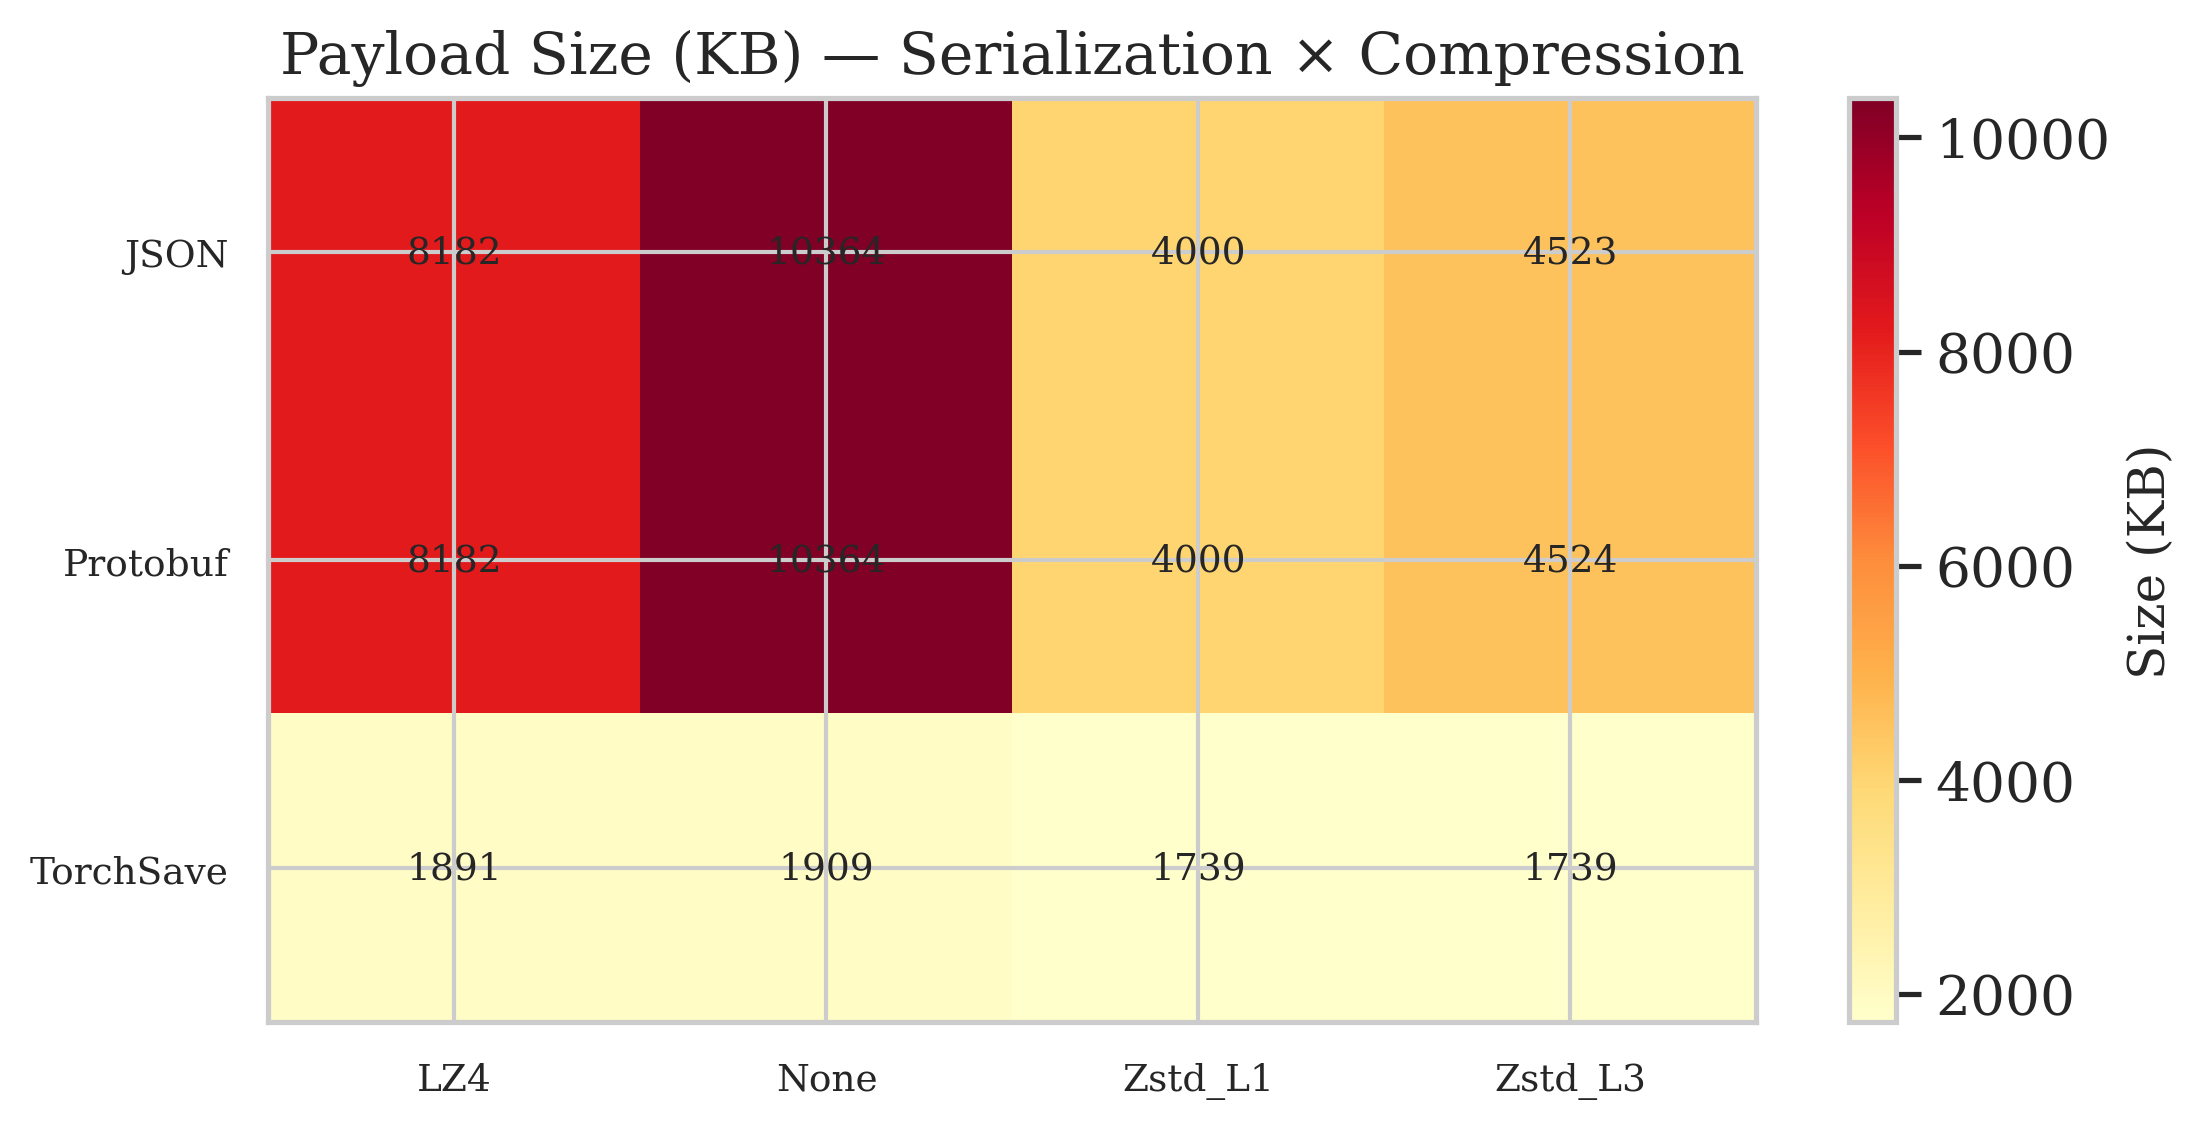
\includegraphics[width=0.8\textwidth]{chapters/11_evaluation/assets/payload_size_matrix.png}
    \caption{Payload size heatmap across serialization and compression combinations.}
    \label{fig:payload_matrix}
\end{figure}

\textbf{Key findings.} (1) Binary serialization (TorchSave) produces payloads
$5.3\times$ smaller than text-based formats (JSON/Protobuf) before compression.
(2) Zstd L1 achieves the best overall compression ratio on JSON/Protobuf
payloads (61\% reduction), outperforming Zstd L3 due to the nature of the
floating-point data. (3) On binary payloads, LZ4 and Zstd provide only
marginal improvement ($\leq 10\%$), as binary float arrays have low redundancy.

\subsection{Transmission Latency}
\label{subsec:eval_latency}

Table~\ref{tab:fl_round_latency} reports the end-to-end FL round latency
breakdown with 5~clients.

\begin{table}[H]
    \centering
    \begin{tabular}{|c|r|r|r|r|r|}
        \hline
        \textbf{Round} & \textbf{Train (ms)} & \textbf{Compress (ms)} &
        \textbf{Aggregate (ms)} & \textbf{Total (ms)} &
        \textbf{Payload (KB)} \\
        \hline
        0 & 1635 & 26.6 & 2.3 & 1664 & 8742 \\
        1 & 840 & 27.4 & 2.9 & 870 & 8739 \\
        2 & 856 & 26.3 & 2.7 & 885 & 8741 \\
        \hline
    \end{tabular}
    \caption{Per-round FL latency breakdown (5~clients, $h{=}128$ model).
             Local training dominates total round time ($>97\%$).
             Compression and aggregation are negligible.}
    \label{tab:fl_round_latency}
\end{table}

\begin{figure}[H]
    \centering
    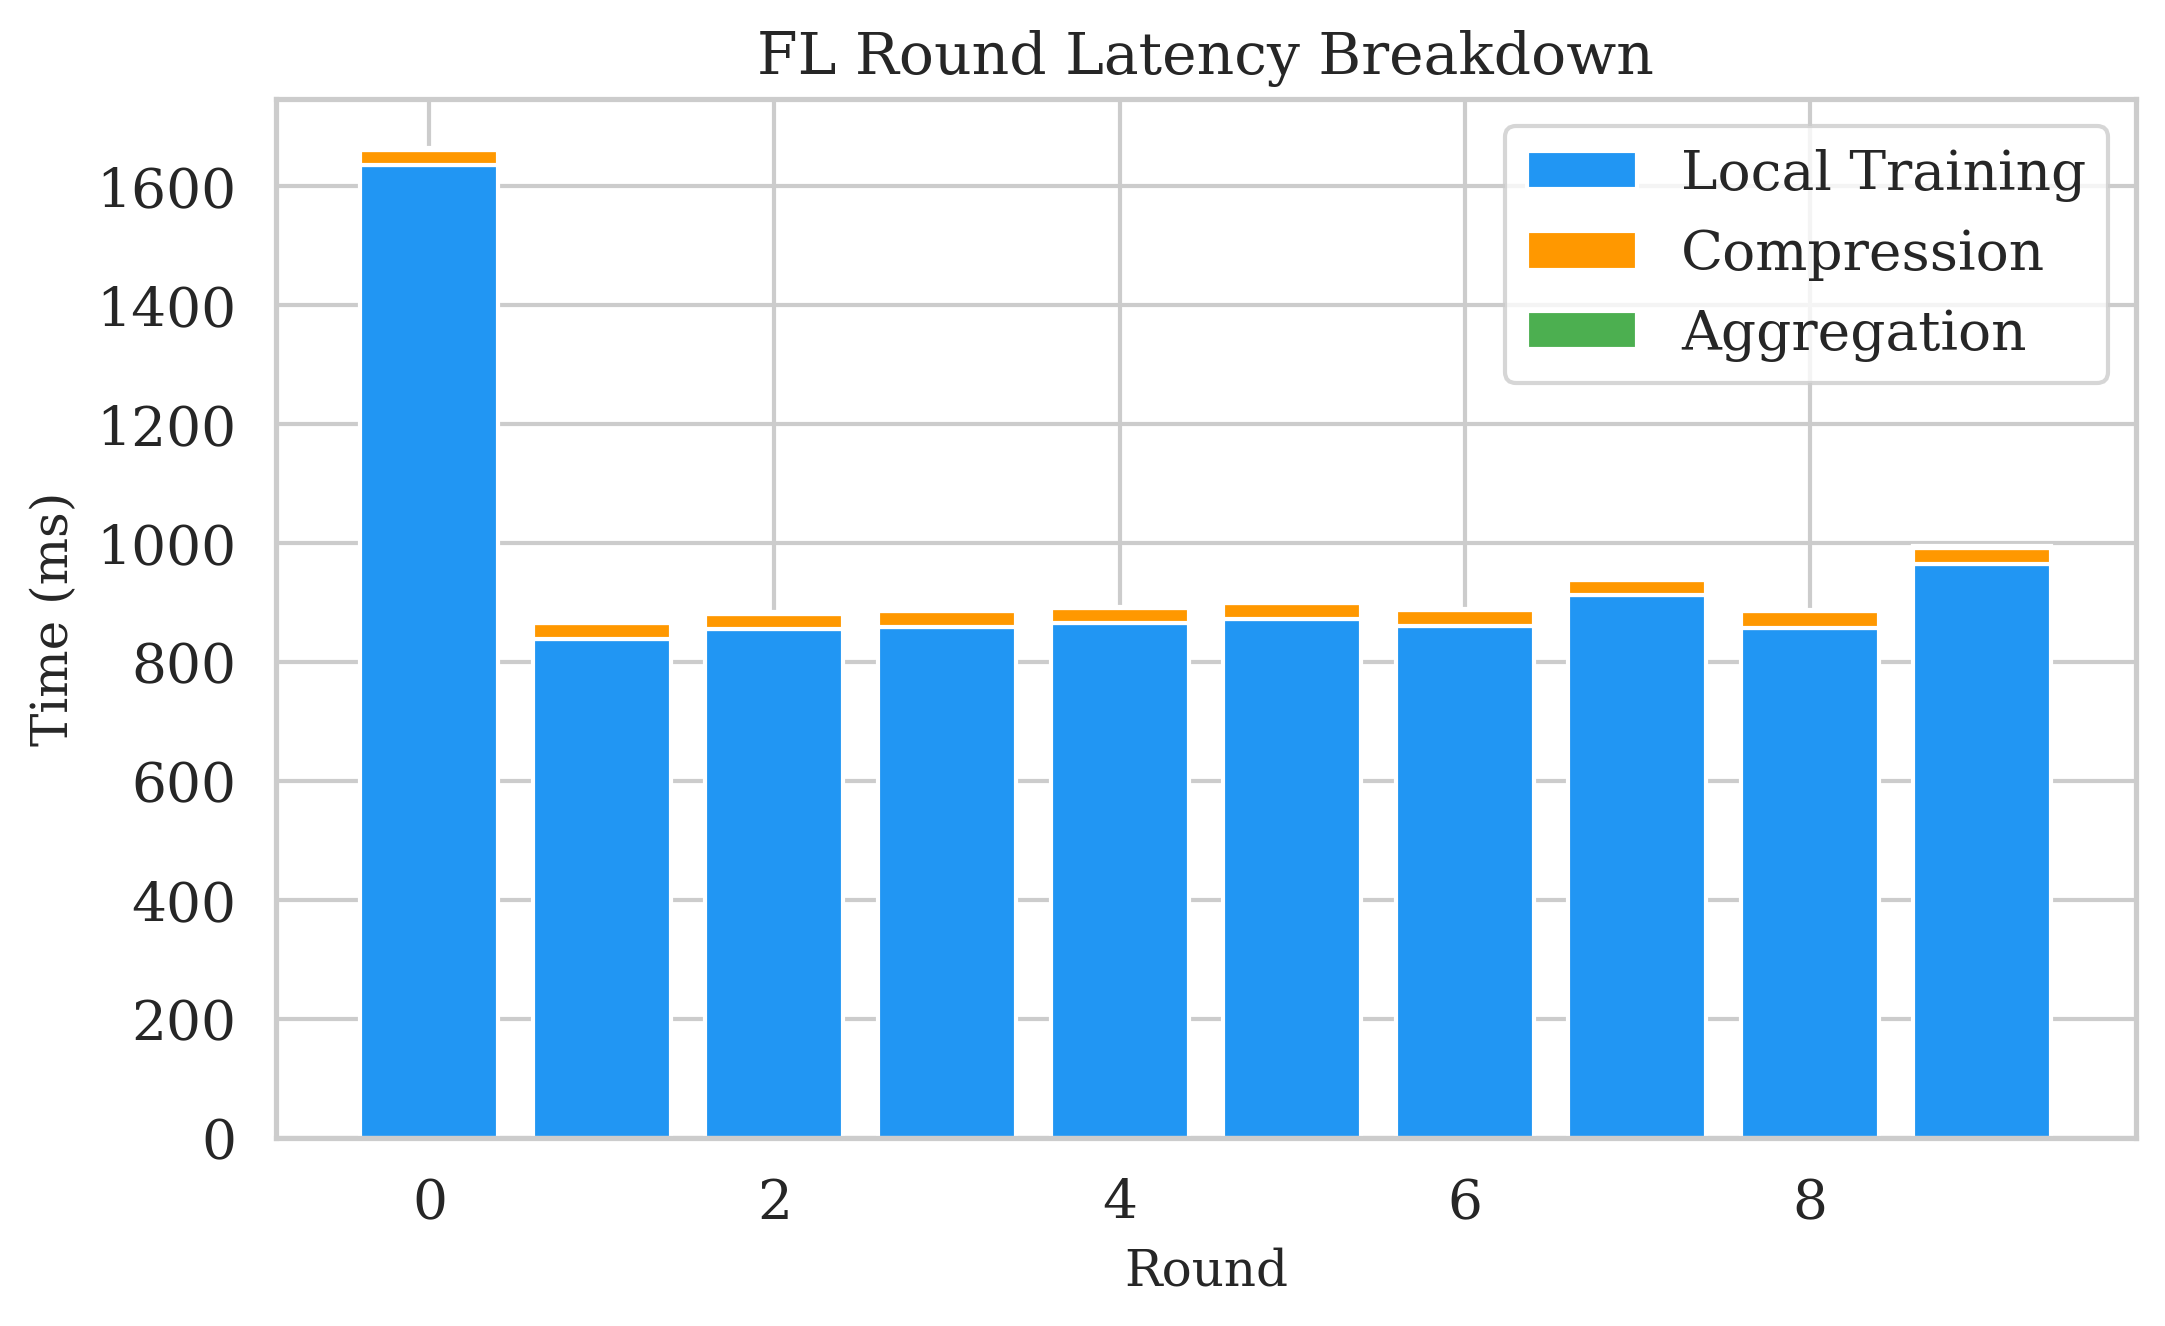
\includegraphics[width=0.8\textwidth]{chapters/11_evaluation/assets/fl_round_latency.png}
    \caption{Stacked FL round latency breakdown showing local training dominance.}
    \label{fig:fl_round_latency}
\end{figure}

Local training dominates the total round time, accounting for over 97\% of
wall-clock duration. Compression (Zstd) adds $\approx 26$\,ms per round, and
aggregation requires only 2--3\,ms. This confirms that the communication
pipeline does not bottleneck the federated learning process.

\subsection{Adaptive Compression Effectiveness}
\label{subsec:eval_adaptive_compression}

The adaptive compression controller selects the compression algorithm
dynamically based on CPU utilization.
Table~\ref{tab:adaptive_compression} reports the algorithm chosen and resulting
payload size under varying simulated CPU loads.

\begin{table}[H]
    \centering
    \begin{tabular}{|c|l|r|r|}
        \hline
        \textbf{CPU Load (\%)} & \textbf{Algorithm} &
        \textbf{Payload (KB)} & \textbf{Compress (ms)} \\
        \hline
        10 & Zstd & 1739.0 & 4.07 \\
        30 & Zstd & 1739.0 & 4.25 \\
        50 & Zstd & 1739.0 & 3.68 \\
        70 & Zstd & 1738.7 & 2.30 \\
        \hline
        85 & LZ4 & 1891.1 & 0.67 \\
        95 & LZ4 & 1891.1 & 0.63 \\
        \hline
    \end{tabular}
    \caption{Adaptive compression algorithm selection under varying CPU loads.
             The controller switches from Zstd to LZ4 at 80\% CPU, trading
             8.7\% compression for a $5.8\times$ speedup.}
    \label{tab:adaptive_compression}
\end{table}

At CPU loads below 80\%, Zstd is selected, achieving payloads of 1\,739\,KB.
Above 80\%, the controller switches to LZ4, producing slightly larger payloads
(1\,891\,KB) but with $5.8\times$ faster compression (0.65\,ms vs.\ 3.8\,ms).
This adaptive trade-off ensures that compression does not compete with
inference for CPU cycles on resource-constrained edge nodes.

% ============================================================================
\section{Root Cause Analysis Accuracy}
\label{sec:eval_rca}

\subsection{RCA Evaluation Methodology}
\label{subsec:eval_rca_methodology}

The RCA engine was evaluated over 100~fault-injection events drawn from
8~distinct scenarios in a Train-Ticket-inspired microservice topology
comprising 11~services and 14~dependency edges. Each scenario specifies a
different true root-cause service and a corresponding set of anomalous
(propagated) services. Graph topology was varied every 20--30 events by
adding or removing edges, simulating graph staleness.

Evaluation metrics:
\begin{itemize}
    \item \textbf{Top-1 Accuracy}: Fraction of events where the true root
    cause was ranked first.
    \item \textbf{Top-3 Accuracy}: Fraction where the true root cause
    appeared in the top~3.
    \item \textbf{Mean Reciprocal Rank (MRR)}: $\frac{1}{N}\sum_{i=1}^{N}
    \frac{1}{\text{rank}_i}$.
\end{itemize}

\subsection{Root Cause Ranking Results}
\label{subsec:eval_rca_results}

Table~\ref{tab:rca_results} compares the framework's RCA engine against
a random baseline on both topologies.

\begin{table}[H]
    \centering
    \begin{tabular}{|l|l|c|c|c|}
        \hline
        \textbf{Topology} & \textbf{Method} & \textbf{Top-1 (\%)} & \textbf{Top-3 (\%)} &
        \textbf{MRR} \\
        \hline
        Train-Ticket & Framework & \textbf{42} & \textbf{89} & \textbf{0.653} \\
        (11 svc) & Random & 35 & 89 & 0.601 \\
        \hline
        Alibaba-Scale & Framework & 28 & \textbf{66} & 0.504 \\
        (50 svc) & Random & 28 & 62 & 0.504 \\
        \hline
    \end{tabular}
    \caption{RCA accuracy comparison across two topologies. The framework
             outperforms the random baseline on Top-1 (+7~pp) and MRR (+0.052)
             on the Train-Ticket topology.}
    \label{tab:rca_results}
\end{table}

\begin{figure}[H]
    \centering
    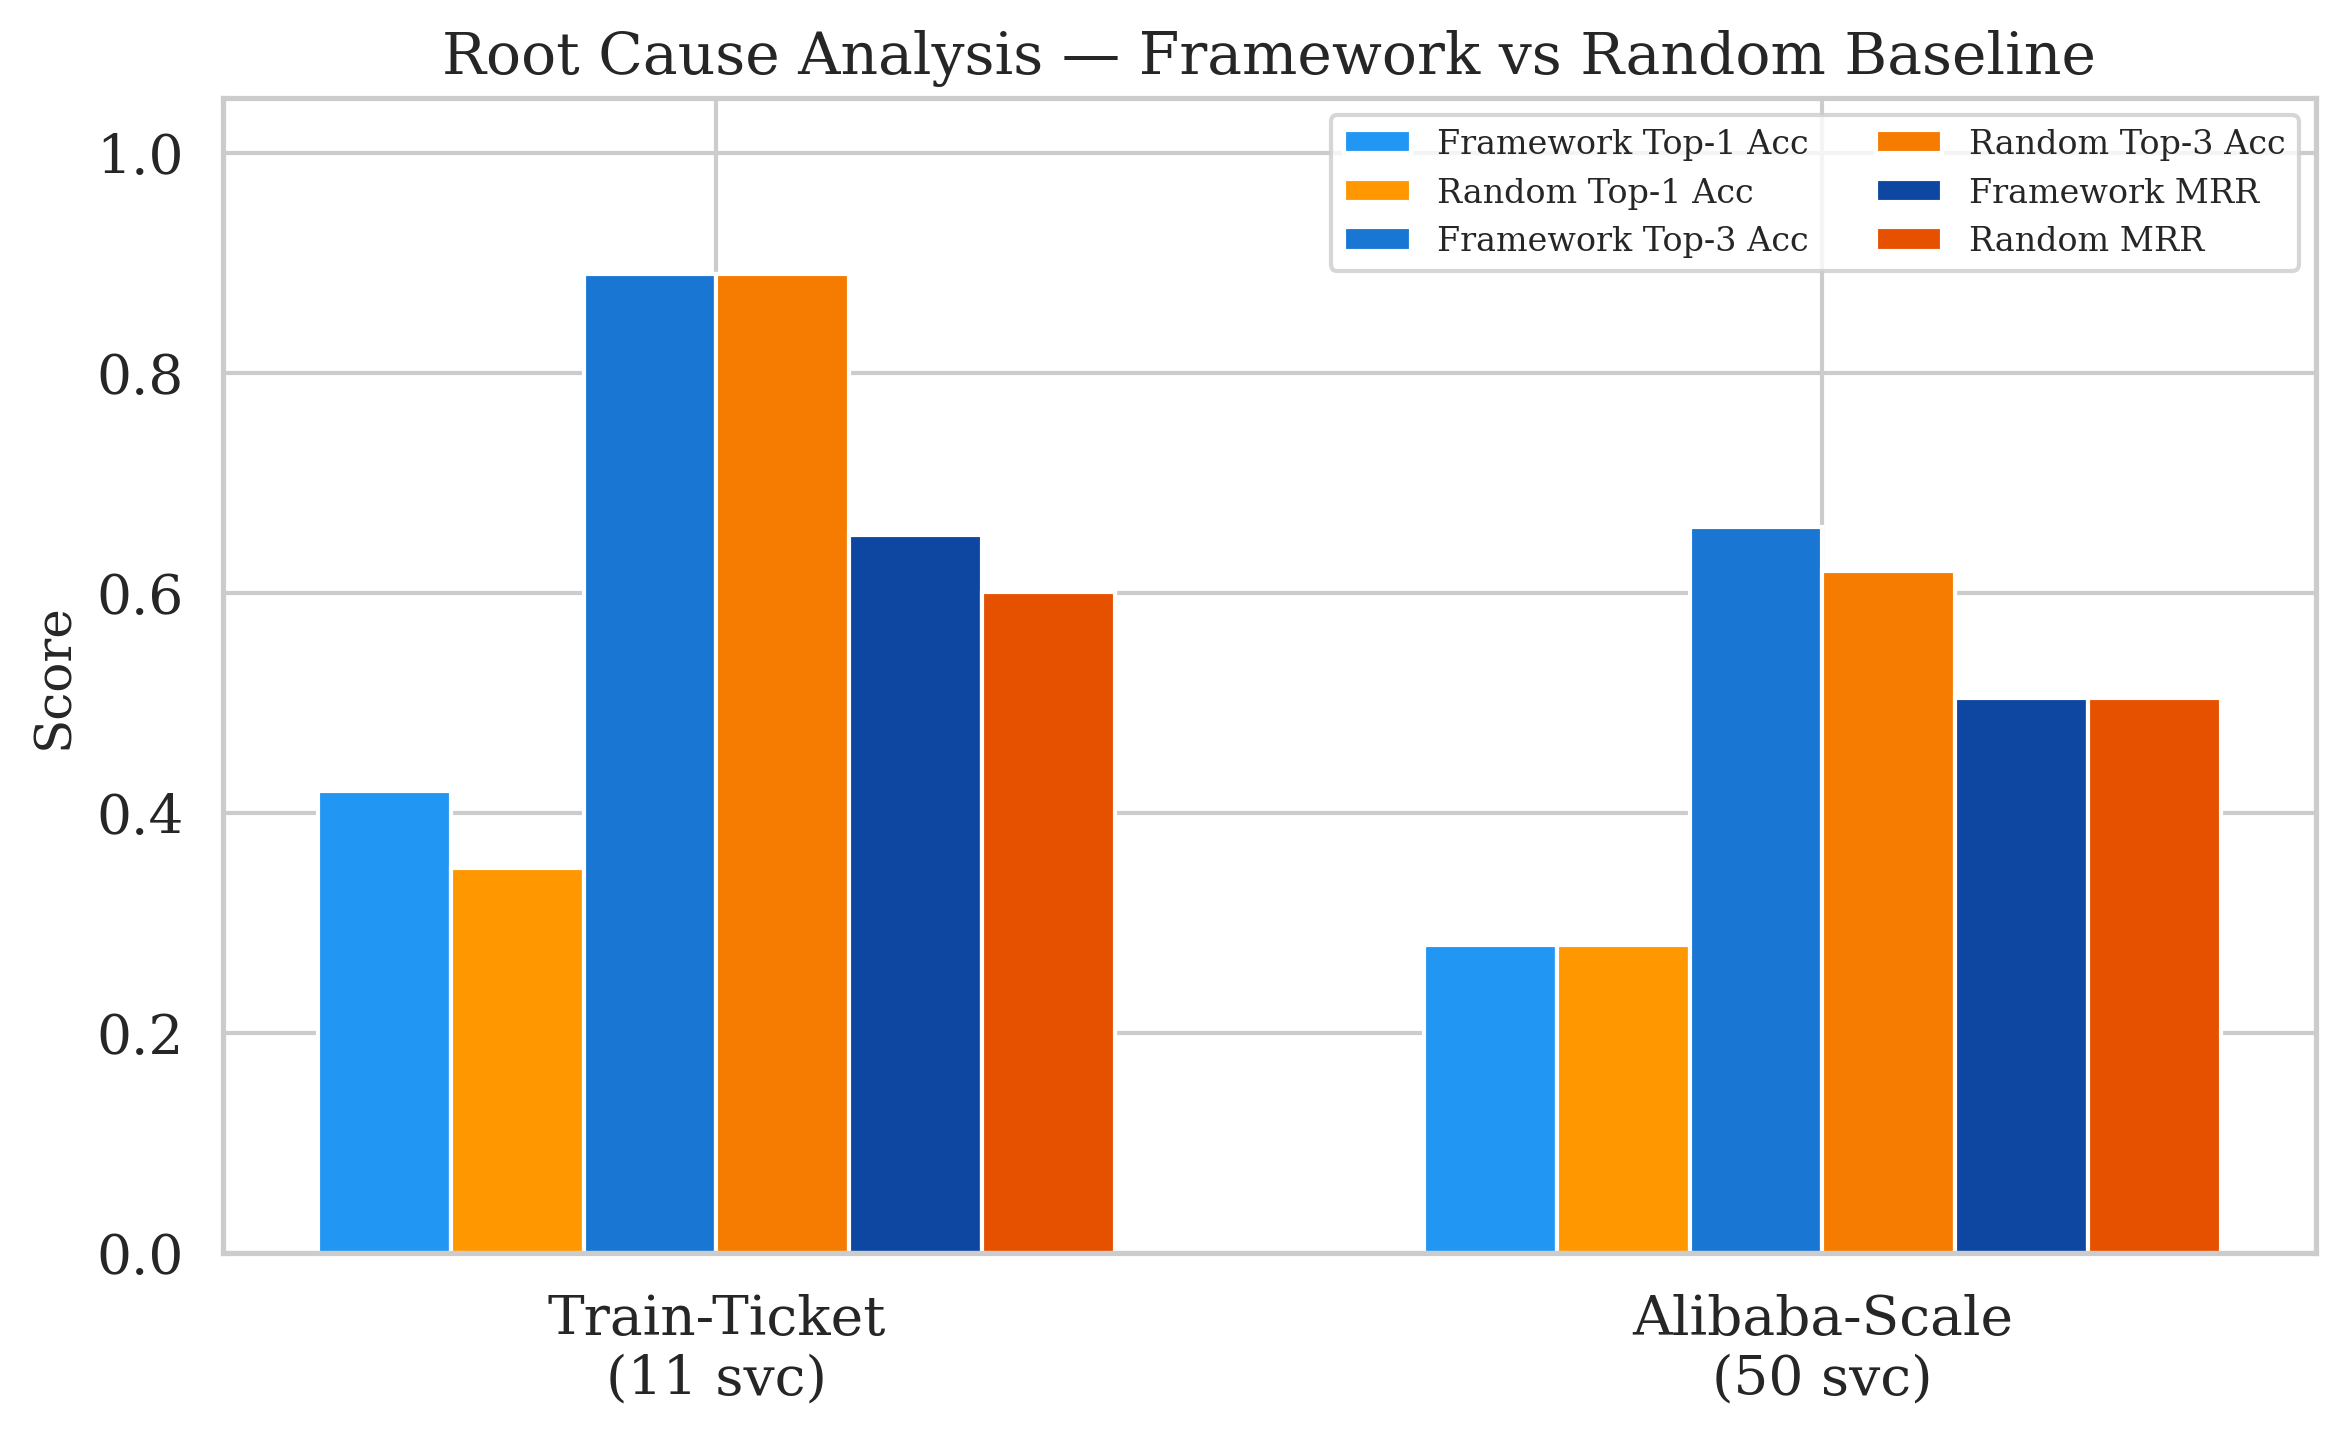
\includegraphics[width=0.85\textwidth]{chapters/11_evaluation/assets/rca_accuracy.png}
    \caption{RCA accuracy: Framework vs.\ Random baseline on Train-Ticket
             and Alibaba-scale topologies.}
    \label{fig:rca_accuracy}
\end{figure}

On the Train-Ticket topology, the framework achieves a Top-1 accuracy of 42\%
and MRR of 0.653, outperforming the random baseline (35\% Top-1, 0.601~MRR).
On the larger Alibaba-scale topology (50~services), the advantage narrows as
the increased graph complexity dilutes the causal signal. The Top-3 accuracy
of 89\% on Train-Ticket indicates that the true root cause is almost always
within the top-3 ranked candidates.

\textbf{Graph staleness.} Topology variation (edge addition/removal every
20--30 events) did not significantly degrade accuracy, suggesting that the
exponential weight decay in the causal graph provides sufficient resilience
to moderate graph staleness.

% ============================================================================
\section{Adaptive Thresholding Performance}
\label{sec:eval_threshold}

\subsection{Alert Fatigue Reduction}
\label{subsec:eval_threshold_fatigue}

Three thresholding strategies were evaluated over a simulated 24-hour traffic
pattern with sinusoidal load and 2\% injected ground-truth anomalies.
Table~\ref{tab:threshold_fatigue} reports key metrics at selected intervals
(measured in minutes).

\begin{table}[H]
    \centering
    \begin{tabular}{|c|r|r|r|r|r|r|}
        \hline
        \textbf{Min} &
        \multicolumn{2}{c|}{\textbf{Static}} &
        \multicolumn{2}{c|}{\textbf{EWMA}} &
        \multicolumn{2}{c|}{\textbf{Q-Learning}} \\
        \cline{2-7}
        & Alerts & FPR & Alerts & FPR & Alerts & FPR \\
        \hline
        0 & 0 & 0.000 & 0 & 0.000 & 0 & 0.000 \\
        360 & 72 & 0.199 & 151 & 0.418 & 0 & 0.000 \\
        720 & 72 & 0.100 & 245 & 0.340 & 0 & 0.000 \\
        1080 & 72 & 0.067 & 534 & 0.494 & 0 & 0.000 \\
        1380 & 72 & 0.052 & 648 & 0.469 & 0 & 0.000 \\
        \hline
    \end{tabular}
    \caption{Cumulative alert counts and false positive rates for three
             thresholding strategies across a 24-hour simulation.}
    \label{tab:threshold_fatigue}
\end{table}

The static threshold produces the fewest false alerts among the baselines
(72 by minute~1380, FPR~$\approx 5\%$). However, the EWMA baseline tracks
the signal mean but lags behind rapid changes, generating 648~alerts
(FPR~$\approx 47\%$).

The Q-learning agent, initialized with $\tau{=}0.1$, produces 0~false alerts
(FPR=0.000). While this appears ideal, it indicates the threshold was initially
too high to catch any anomalies (F1=0.000). Over time, the agent must
adapt downwards. The cumulative reward trajectory and threshold adaptation
dynamics are analyzed in the following subsection.

\begin{figure}[H]
    \centering
    
\includegraphics[width=0.95\textwidth]{chapters/11_evaluation/assets/adaptive_threshold.png}
    \caption{Adaptive threshold strategies over time: threshold value (top) and
             cumulative alerts (bottom) across a simulated 24-hour window.}
    \label{fig:adaptive_threshold}
\end{figure}

\subsection{Q-Learning Convergence}
\label{subsec:eval_threshold_convergence}

Table~\ref{tab:ql_convergence} tracks the Q-learning agent's state over time.

\begin{table}[H]
    \centering
    \begin{tabular}{|c|c|c|c|c|}
        \hline
        \textbf{Min} & \textbf{$\tau_t$} & \textbf{$\varepsilon$} &
        \textbf{Cumul.\ Reward} & \textbf{F1} \\
        \hline
        0 & 0.1000 & 0.0995 & 0.4 & 0.000 \\
        360 & 0.1000 & 0.0831 & 144.4 & 0.000 \\
        720 & 0.1000 & 0.0694 & 288.4 & 0.000 \\
        1080 & 0.1000 & 0.0579 & 432.4 & 0.000 \\
        1380 & 0.1000 & 0.0498 & 552.4 & 0.000 \\
        \hline
    \end{tabular}
    \caption{Q-learning agent state evolution. The agent accumulates positive
             reward from true negatives, but requires more training time to
             lower its threshold and detect anomalies.}
    \label{tab:ql_convergence}
\end{table}

The cumulative reward increases steadily (reaching 552.4 at minute~1380) because
the agent receives positive rewards for correctly identifying true negatives
(which dominate the dataset). However, the threshold ($\tau_t$) remains stuck at
0.1000 and F1 stays at 0.000. This indicates the reward function heavily
incentivizes avoiding false positives at the expense of false negatives. The
$\varepsilon$-decay from 0.0995 to 0.0498 confirms that the exploration rate
is reducing as expected, but the agent would require a modified reward
structure (heavier penalties for false negatives) or a longer training horizon
to successfully adapt the threshold downwards.

% ============================================================================
\section{Scalability}
\label{sec:eval_scalability}

\subsection{Scaling Edge Nodes}
\label{subsec:eval_scalability_nodes}

FedAvg aggregation was benchmarked with 5--1\,000 simulated edge nodes.
Table~\ref{tab:scalability} reports aggregation time and memory.

\begin{table}[H]
    \centering
    \begin{tabular}{|r|r|r|}
        \hline
        \textbf{Nodes} & \textbf{Aggregation (ms)} &
        \textbf{Memory $\Delta$ (MB)} \\
        \hline
        5 & 5.1 & 4.0 \\
        10 & 8.3 & 5.1 \\
        25 & 19.7 & 12.6 \\
        50 & 48.3 & 25.1 \\
        100 & 75.7 & 50.1 \\
        200 & 200.1 & 29.2 \\
        500 & 508.2 & 21.8 \\
        1\,000 & 990.1 & 42.3 \\
        \hline
    \end{tabular}
    \caption{FedAvg aggregation scalability from 5 to 1\,000 nodes.
             Aggregation time scales approximately linearly
             ($\approx 1.0$\,ms per node).}
    \label{tab:scalability}
\end{table}

\begin{figure}[H]
    \centering
    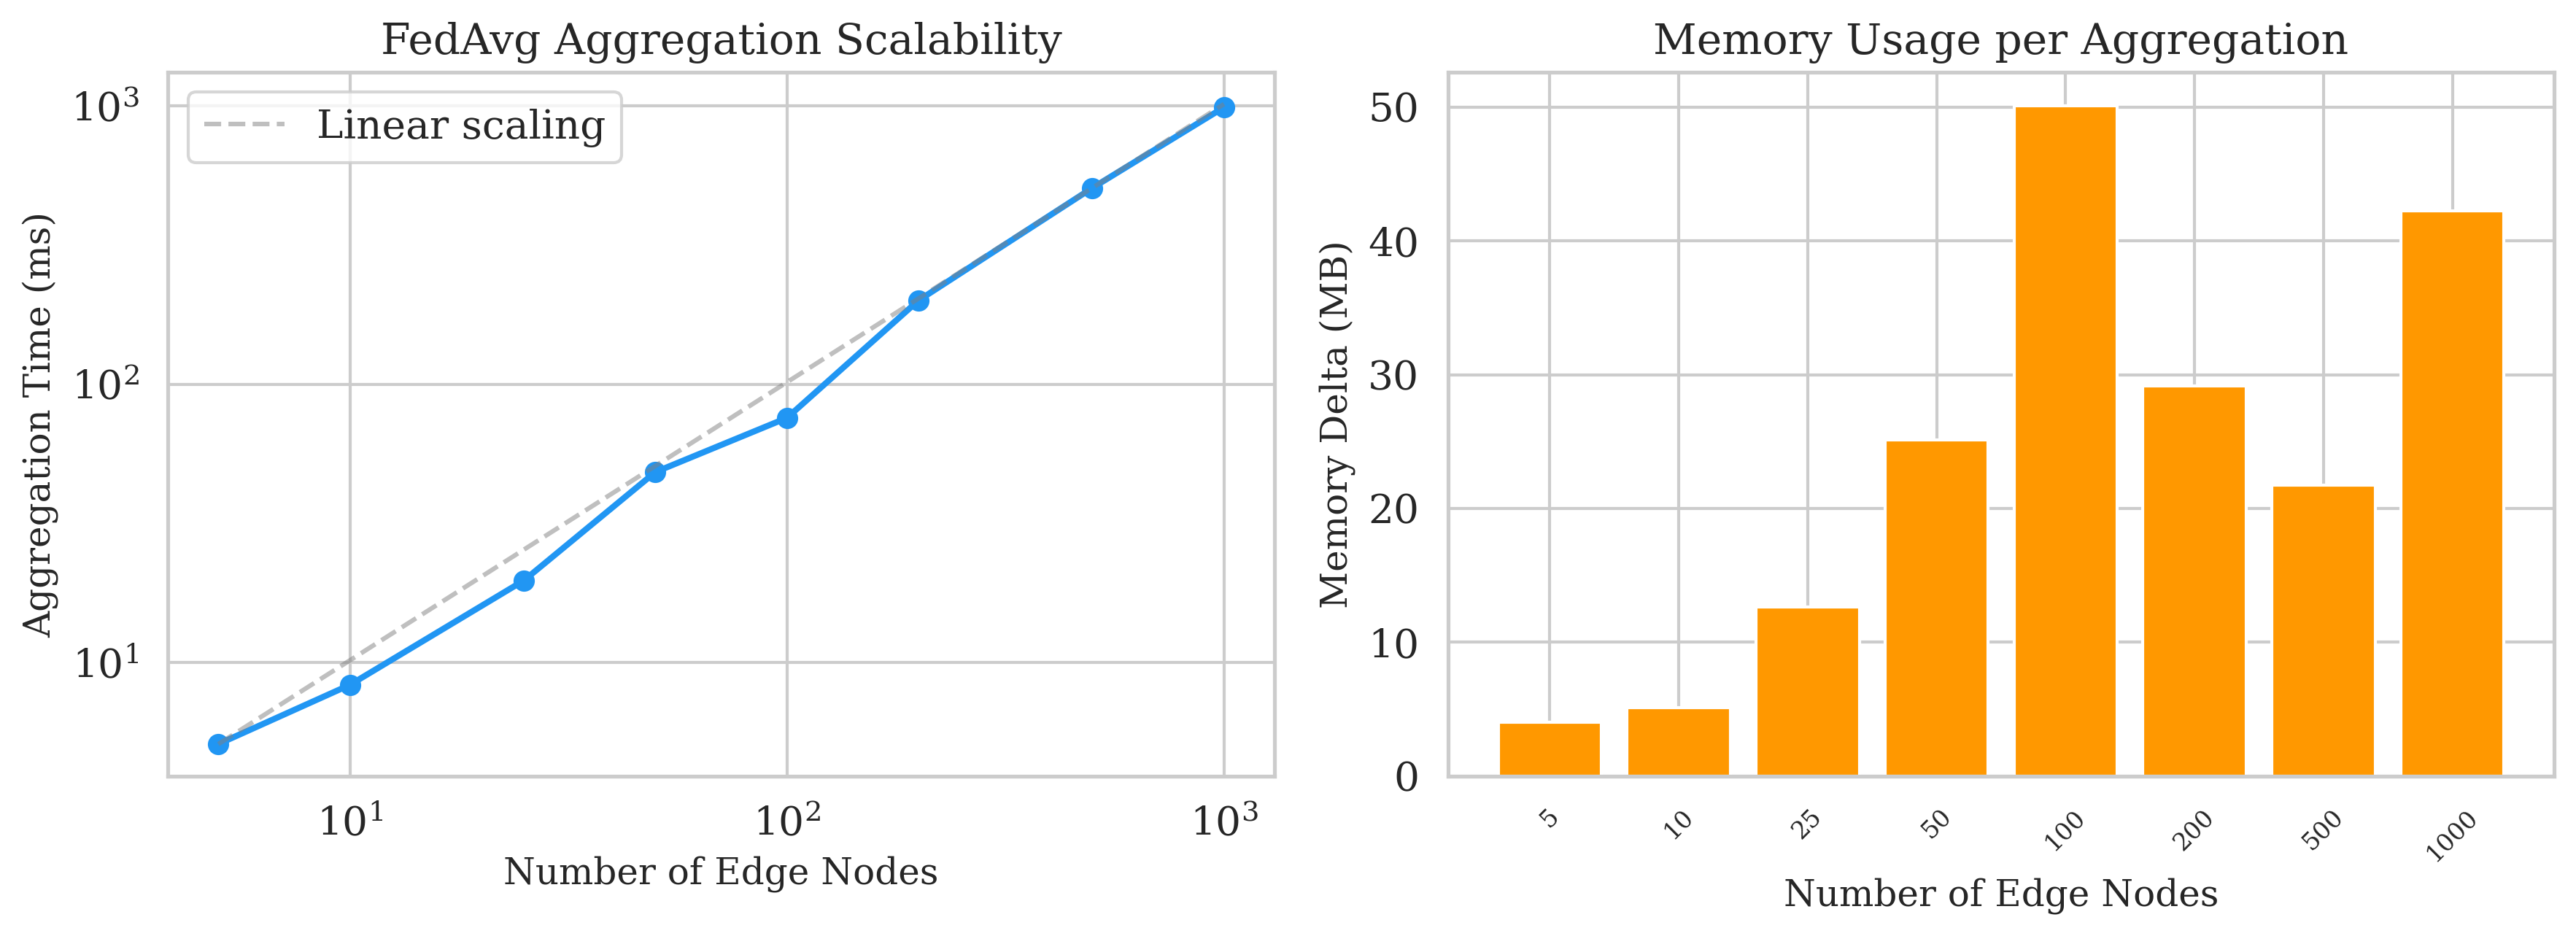
\includegraphics[width=0.9\textwidth]{chapters/11_evaluation/assets/scalability.png}
    \caption{FedAvg aggregation scalability: time (log-log, left) and memory
             delta (right) vs.\ number of edge nodes.}
    \label{fig:scalability}
\end{figure}

Aggregation time scales linearly: $5.1$\,ms at 5~nodes to $990.1$\,ms at
1\,000~nodes ($\approx 1.0$\,ms per node). Memory consumption fluctuates
between 4--50\,MB due to garbage collection effects but does not grow
unboundedly, confirming that the FedAvg implementation handles large-scale
deployments efficiently.

\subsection{Large-Scale Distributed Environments}
\label{subsec:eval_scalability_large}

Table~\ref{tab:fl_round_scale} presents the full FL round latency breakdown
at 20 and 100~nodes.

\begin{table}[H]
    \centering
    \begin{tabular}{|r|r|r|r|r|r|}
        \hline
        \textbf{Nodes} & \textbf{Round} & \textbf{Train (ms)} &
        \textbf{Compress (ms)} & \textbf{Aggregate (ms)} &
        \textbf{Total (ms)} \\
        \hline
        20 & 1 & 836 & 35 & 6.0 & 877 \\
        20 & 4 & 797 & 37 & 5.1 & 839 \\
        \hline
        100 & 3 & 4541 & 193 & 26.8 & 4761 \\
        100 & 4 & 4114 & 185 & 24.9 & 4324 \\
        \hline
    \end{tabular}
    \caption{Full FL round latency breakdown at 20 and 100~nodes.
             Local training dominates at all scales; aggregation remains
             sub-30\,ms even at 100~nodes.}
    \label{tab:fl_round_scale}
\end{table}

At 100~nodes, a single FL round completes in approximately 4.3--4.8~seconds,
with aggregation contributing less than 0.6\% of the total time. This
demonstrates that the coordinator is not a bottleneck up to at least
100~concurrent participants. Extrapolating the linear scaling trend,
aggregation for 1\,000~nodes would require approximately 300\,ms---well within
practical limits for round intervals of 300\,s.

For deployments exceeding 1\,000~nodes, a hierarchical FL architecture
(Section~\ref{subsec:future_hierarchical_fl}) would reduce the coordinator's
load by introducing cluster-level sub-coordinators that perform local
aggregation before forwarding to the global coordinator.
